\chapter*{Appendix}
\addcontentsline{toc}{chapter}{Appendix}
\section*{List of appendices}
\vspace{-8em}

% vor \listofanhang müssen Einrückungen angepasst werden
\abstaendeanhangverzeichnis

\listofanhang
\clearpage
\spezialkopfzeile{Attachement} % damit in der Kopfzeile das Wort "Anhang" angezeigt wird

\anhang{So funktioniert's}

\lstset{language=TeX, % hervorzuhebende Keywords definieren
  morekeywords={anhang, anhangteil}
}


Um den Anforderungen der Zitierrichtlinien nachzukommen, wird das Paket \verb|tocloft| verwendet. Jeder Anhang wird mit dem (neu definierten) Befehl \lstinline|\anhang{Bezeichnung}| begonnen, der insbesondere dafür sorgt, dass ein Eintrag im Anhangsverzeichnis erzeugt wird. Manchmal ist es wünschenswert, auch einen Anhang noch weiter zu unterteilen. Hierfür wurde der Befehl \lstinline|\anhangteil{Bezeichnung}| definiert.

\anhang{House of Prototyping Guidelines: Prototyping Dimensions}\label{attachement:prototyping_dimensions}
\begin{figure}[htb]
\centering
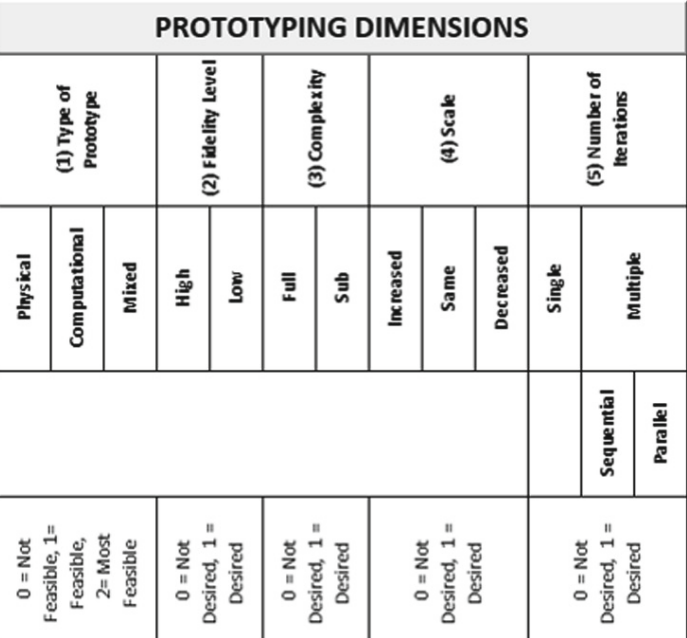
\includegraphics[width=0.9\linewidth]{graphics/Prototyping_dimensions.png}
\caption{Prototyping Dimensions to categorize prototypes}
\end{figure}

\anhang{Weight matrix within the Hopfield Network}\label{attachement:weight_matrix}
\begin{lstlisting}
def initialize_weights_and_biases(self, components):
  num_hidden = self.num_hidden_neurons
  num_visible = self.num_visible_neurons

  #Result size: 100,64

  # Initialize a symmetric weight matrix for simplicity
  self.weights = np.zeros((num_hidden + num_visible, num_hidden + num_visible))

  # Fill in the weights from components for connections between hidden and visible layers
  # for connections between hidden and visible layers
  for i in range(num_hidden):  # Looping through hidden neurons
      for j in range(num_visible):  # Looping through visible neurons
          hidden_index = i
          visible_index = j + num_hidden

          # Additional safeguard: Ensure 'j' is within the bounds of 'components' second dimension
          if j < len(components[0]):
              self.weights[hidden_index, visible_index] = components[i][j]
              self.weights[visible_index, hidden_index] = components[i][j]
          else:
              print(f"Attempted to access components[{i}][{j}], which is out of bounds.")

  return self.weights
\end{lstlisting}

